%! Author = Len Washington III
%! Date = 10/2/24

% Preamble
\documentclass[
	% author={}, % Remove the percentage sign and add your name within the brackets.
	number={5},
]{math486homework}

% Document
\begin{document}

\maketitle

\begin{problems}
	\problem Strep throat, sinus infections, etc. usually require an antibiotic to help bring the infection under control.
	Zithromax (azithromycin) is often prescribed for these infections as a Z Pak containing 6 pills.
	Suppose we design a two compartment model for Zithromax with the first compartment being the GI tract $x(t)$ and the second compartment being the blood stream, $y(t)$ with the following system of ODE's:
	\begin{equation*}
	\begin{aligned}
		x' &= -k_{1}x + I(t)\\
		y' &= k_{1}x - k_{2}y\\
	\end{aligned}
	\end{equation*}
	where $I(t)$ is the input of the pills.
	The initial amount in each compartment equal to 0.
	The dosing regimen for a Z Pak is 2 pills the first day and then 1 pill for the following 4 days (5 day regimen).
	The time between the doses is 1 day and each pill delivers $D$ units of the drug.
	\begin{problems}
		\subproblem Find the amount of the drug in each compartment from days 1 to 8.
		Model each pill dose by a Dirac delta function spiked at the appropriate time. \addanswer{Problem-1a}
		\subproblem If each pill is 400mg, $k_{1} = 0.9$, and half-life of the drug in the blood is 2.3 days, graph $x(t)$ and $y(t)$ on the same axes from day 1 to day 8. \addanswer{Problem-1b}
	\end{problems}
	\problem Consider a system of ODE's with initial conditions.
	\begin{equation}
		\frac{d\vec{x}}{dt} = A\vec{x} + \vec{b} = \left[ \begin{array}{cc}
			-2 & 1\\
			1 & -2
		\end{array} \right]\vec{x} + \left[ \begin{array}{c}
			3\\
			-1
		\end{array} \right], \vec{x}(0) = \left[ \begin{array}{c}
			2\\
			2
		\end{array} \right]
		\label{eq:1}
	\end{equation}
	Answer~\ref{prb:2a}-\ref{prb:2d} on paper using matrix methods.
	\begin{problems}
		\subproblem Find a fundamental set of solutions to the associated homogenous equation. \addanswer{Problem-2a}
		\subproblem Find a particular solution $x_{p}(t)$ using undetermined coefficients, i.e. just guess a constant solution. \addanswer{Problem-2b}
		\subproblem Form the general solution and then find the specific solution of the initial value problem. \addanswer{Problem-2c}
		\subproblem Describe the behavior at $t\rightarrow\infty$. \addanswer{Problem-2d}
		\subproblem Use the \textit{Mathematica} \hyperref[fig:mathematica]{notebook} attached for the following questions:
		\begin{figure}[H]
			\centering
			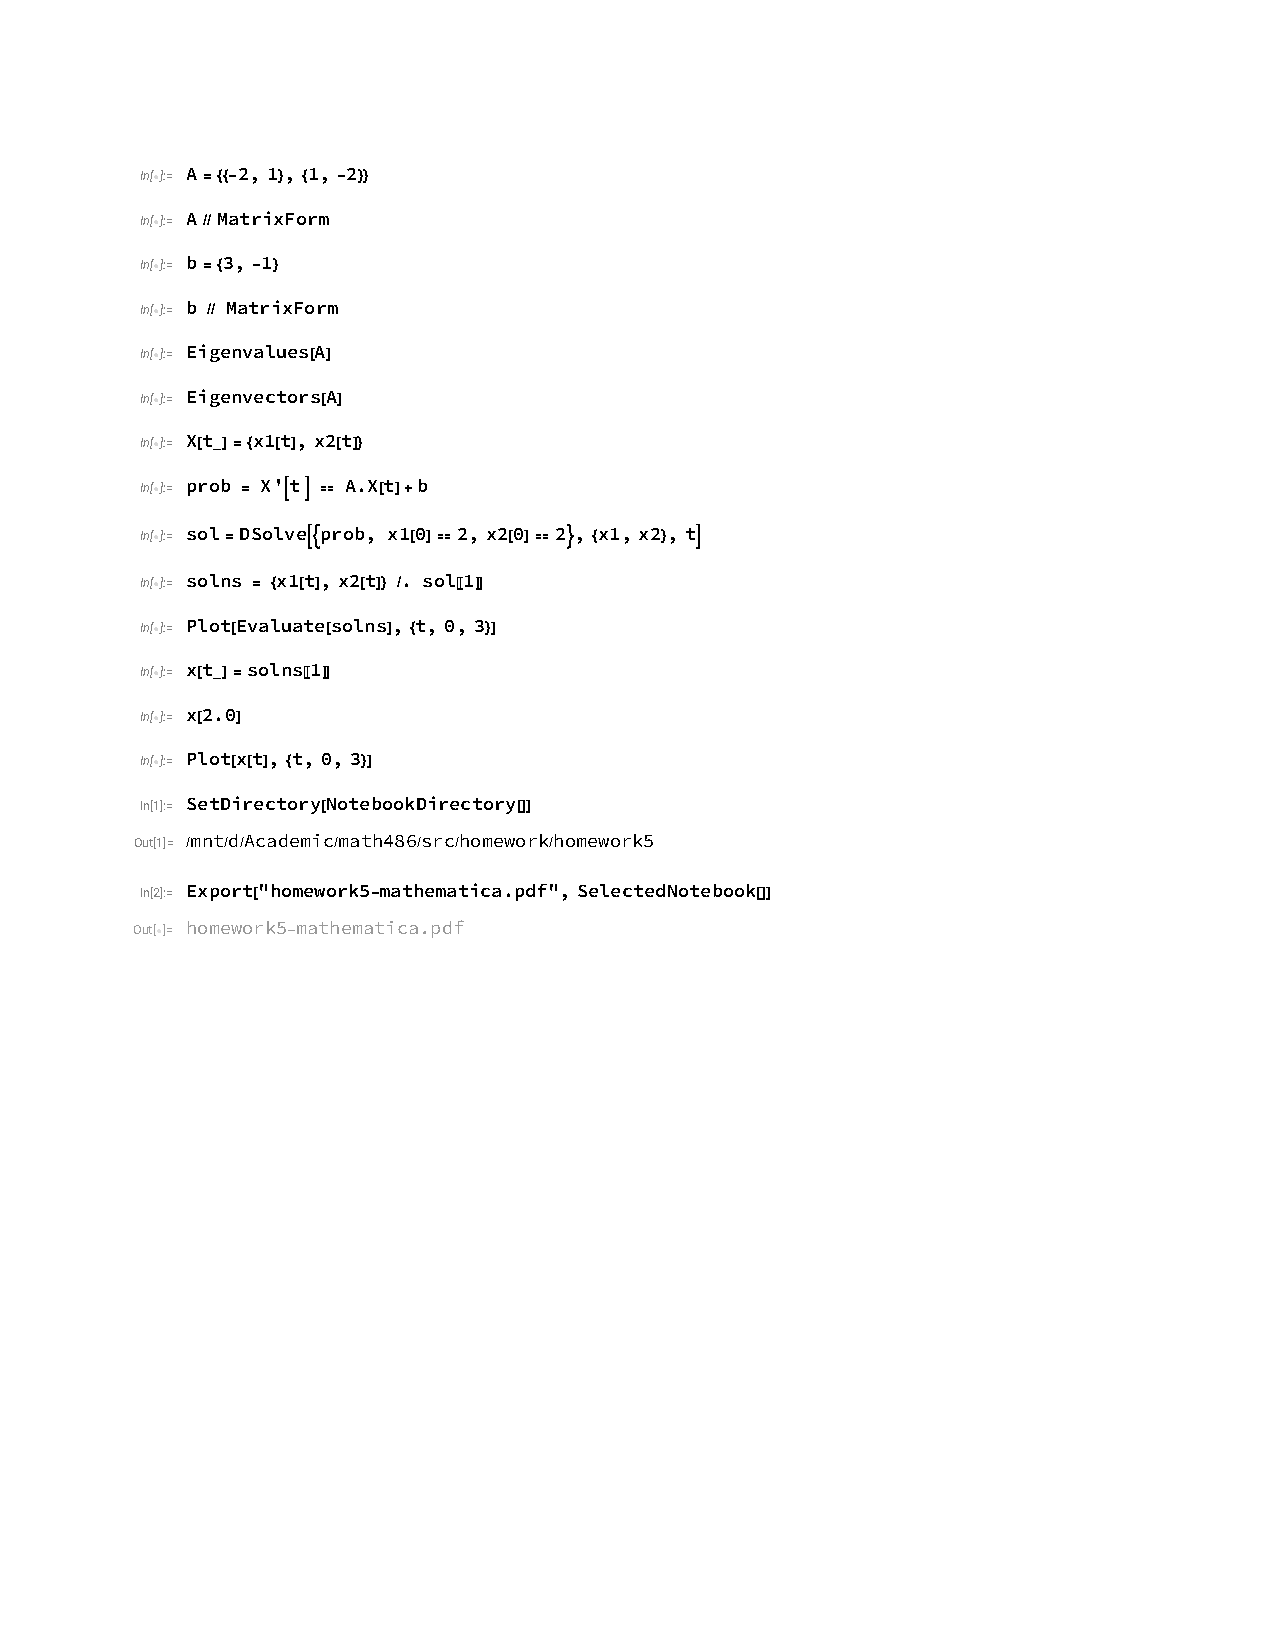
\includegraphics[width=\textwidth]{homework5/homework5-mathematica}
			\caption{Mathematica notebook}
			\label{fig:mathematica}
		\end{figure}
		\begin{problems}
			\subsubproblem Find the eigenvalues and eigenvectors of the coefficient matrix $A$.
			Do they agree with your hand calculation? \addanswer{Problem-2e-i}
			\subsubproblem Use DSolve to construct the solution~\eqref{eq:1}. \addanswer{Problem-2e-ii}
			\subsubproblem Graph $x_{1}(t)$ and $x_{2}(t)$ for $0 \leq t \leq 3$ on the same axes. \addanswer{Problem-2e-iii}
		\end{problems}
	\end{problems}
	\problem In the lecture, a lead uptake model discussed as is a 3 compartment model with compartments - plasma, soft tissue and bones.
	The amount of lead in the compartments is measured in micrograms and time is measured in days.
	Let $x_{1}(t)$ be the amount in the blood, $x_{2}(t)$ is the amount in the soft tissues, and $x_{3}(t)$ is the amount in the bones.
	The following data was given in Rabinowitz, Wetherill, and Kopple, \textit{Science}, \textbf{182}, 1973, pp. 725-727:
	\begin{equation}
		\begin{aligned}
			k_{01} &= 0.0211 \sep k_{21} &= 0.0111 \sep k_{31} &= 0.0039\\
			k_{02} &= 0.0162 \sep k_{12} &= 0.0124 \sep k_{13} &= 0.000035
		\end{aligned}
		\label{eq:2}
	\end{equation}
	Note: You cannot do this problem by hand (easily) so use Mathematica or equivalent.
	The Mathematica notebook from problem 1 should help.
	\begin{problems}
		\subproblem Re-derive the system of ODE's $\frac{d\vec{x}}{dt} = A\vec{x} + \vec{I}$ for the amount in each compartment based on the figure in the notes, i.e. check to make sure the equations in the lecture notes are correct.\addanswer{Problem-3a}
		\subproblem Again assume $I=0$ but now $x_{1}(0)=0$, $x_{2}(0)=0$, and $x_{3}(0)=6$:
		\begin{problems}
			\subsubproblem Construct the solution of the system of ODE's. \addanswer{Problem-3b-i}
			\subsubproblem Graph the three amounts in the different compartments on the different axes for 1000 days. \addanswer{Problem-3b-ii}
			\subsubproblem By using the graph of $x_{3}(t)$, estimate the initial half-life $\tau_{1/2}$ in days for the amount of leads in the bones, i.e. how long to go from $x_{3}(0) = 6$ to $x_{3}(\tau_{1/2}) = 3.$
			You may need to increase the time range.
			Can you obtain an analytic estimate for the half-life?\addanswer{Problem-3b-iii}
		\end{problems}
		\subproblem Suppose there is a drug that speeds the removal of lead from the bones such that the removal rate $k_{13}$ is tripled.
		Re-do steps~\ref{prb:3bi}-\ref{prb:3biii} in part~\ref{prb:3b}.
		Compare the results in~\ref{prb:3b} and~\ref{prb:3c}.\addanswer{Problem-3c}
	\end{problems}
\end{problems}

\end{document}